\chapter{Aufbau \gls{programname}}
\label{ch:aufbau_programname}
                                        TODO:
                                        graph package image einfügen? quer? view image quer? text davor oder danach? mit sidewaysfigure wird die section auf eine eigene seite gestellt.
                                        gleiches bei marks sqdiag beachten, das addpckdata.
                                        die unteren 2 Packages noch beschreiben.
                                        Korrekturlesen.
\section{Architekturbeschreibung}
Im Groben gehalten funktioniert der Daten- und Befehlsfluss im Trufflehog-Entwurf
wie im klassischen \gls{mvc}. Der Presenter aktiviert Services, welche das Model basierend
auf empfangenem Netzwerkverkehr verändert und das View aktualisiert sich am Model.
Da viele Threads im Programm parallel arbeiten aber dennoch kommunizieren müssen,
verlassen wir uns an einigen Stellen auf das \gls{observerpattern} mit
Threadsicheren Datenstrukturen.\newline
\newline

\section{Paketbeschreibung}

\begin{frame}{command}
    \begin{figure}
    	\centering
    	\includegraphics[width=\textwidth]{./images/command.png}
    \end{figure}
\end{frame}


\begin{frame}{service}
    \begin{figure}
    	\centering
    	\includegraphics[width=\textwidth]{./images/service.png}
    \end{figure}
\end{frame}
 \begin{frame}{service}
    \begin{itemize}[<+->]
      \item Aufgaben
        \begin{itemize}
          \item Daueraufgaben von TruffleHog
          \item Interprozesskommunikation
          \item Commands ausführen
          \item Replay-Funktion bereitstellen
        \end{itemize}
      \item Entwurfsentscheidung
        \begin{itemize}
          \item Einmaliger Aufruf
          \item Eigenständiges Arbeiten
          \item Laufen in eigenem Thread
        \end{itemize}
    \end{itemize}
\end{frame}

\subsection{util}
\label{subsec:util}

\begin{figure}[H]
  \centering
  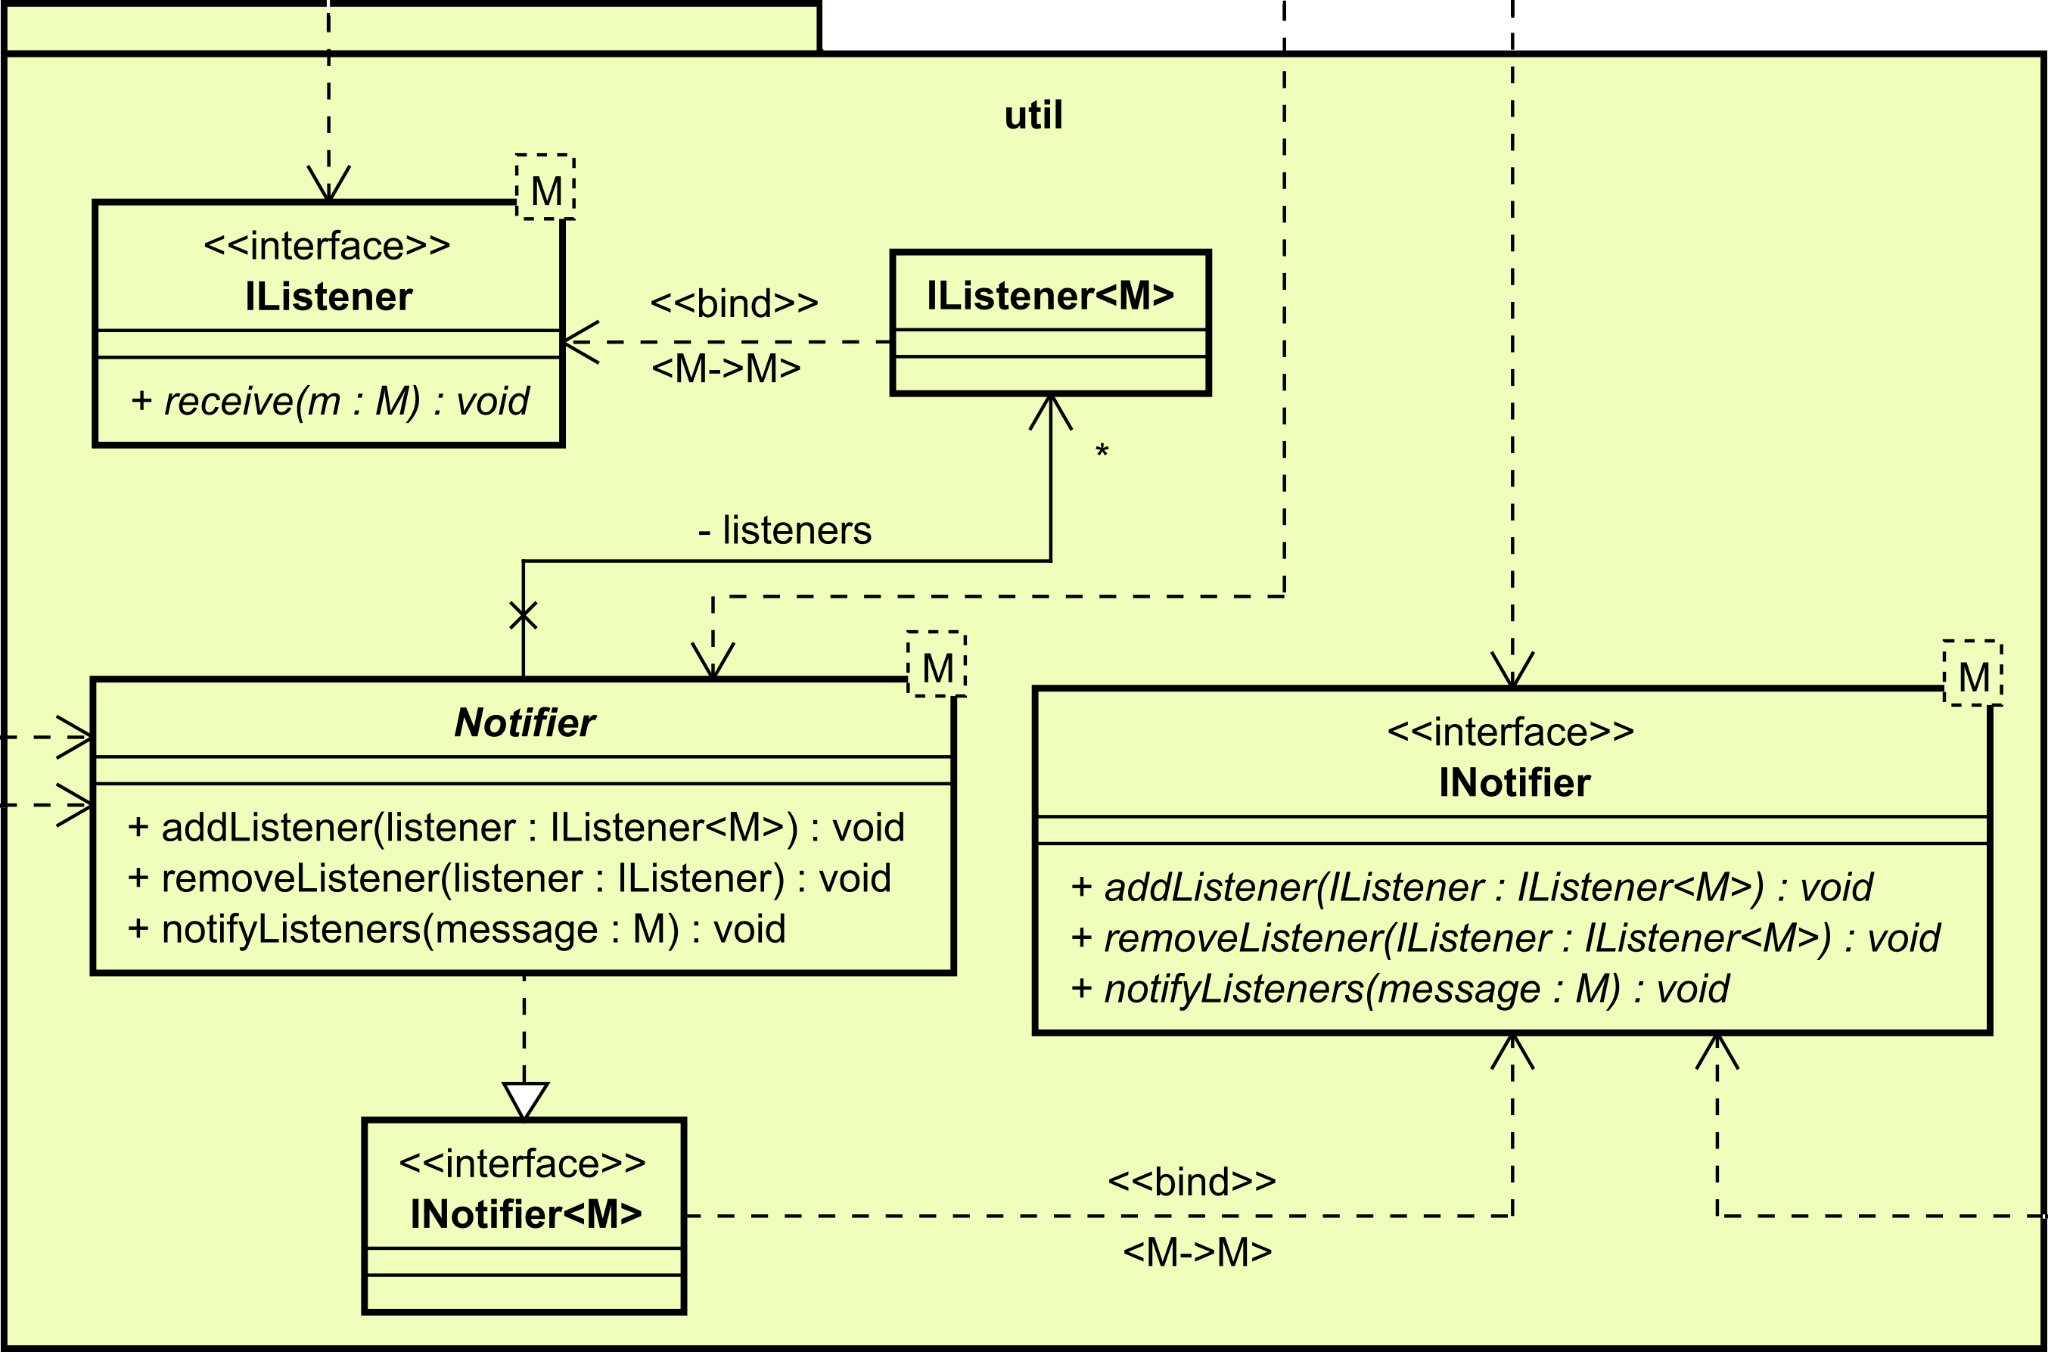
\includegraphics[width=\textwidth]{../diagramimages/util.png}
  \caption{util-Package}
\end{figure}

\medskip
Im util-Package befinden sich Klassen, die komplett von \gls{programname} abgekoppelt
sind. D.h. sie werden nur als Ressource, wie eine Liste, benutzt und nehmen kein
Bezug auf das Programm.\newline
Konkret befinden sich 3 Klassen im util-Package, die alle zusammen eine
Variation des \gls{observerpattern}s realisieren. Der \textit{Notifier} ist dazu da
ein beliebiges Objekt zu verschicken, deshalb der Generic. Er ist das Subjekt aus
dem \gls{observerpattern}.
\newline
\newline
Der \textit{INotifier} existiert für den Fall, dass ein
Objekt ein Notifier sein muss, aber nicht Notifier vererben kann, weil es
schon eine andere Klasse bererbt. Dieses Problem tritt beispielsweise im
\hyperref[subsec:view]{view}-Package auf, wo viele Klassen \gls{gui}-Aktionen als Commands
gekapselt an den Executor verschicken und gleichzeitig JavaFX Klassen bererben müssen.
Um dieses Problem zu lösen implementieren diese Klassen das INotifer-Interface
und haben ein Hilfsobjekt, das Notifier vererbt um somit die gewünschte Funktionalität zu
bieten.
\newline
\newline
Der \textit{Listener} ist der Beobachter aus dem \gls{observerpattern}. Hier ist nichts
besonders vaiiert worden, mit Ausnahme der receive-Methode, bei der wir einen Parameter eingeführt
haben damit der Listener das versendete Objekt des \gls{notifier}s auch empfangen kann.
Zu diesem Zweck existiert auch wieder ein Generic.
\newline
\newline
Dieses \gls{observerpattern} verwaltet das Verschicken und Empfangen von Commands in
\gls{programname}. In anderen Worten, jede Klasse, die Commands verschickt, ist ein
\gls{notifier}, und jede Klasse, die Commands empfängt, ist ein \gls{listener}. Dieses Design
hat große Vorteile, da die Sender und die Empfänger komplett voneinander abgekoppelt
sind. Der \hyperref[subsec:presenter]{Presenter} registriert die \gls{listener} bei Programmstart
bei den \gls{notifier}n, somit kennt der \gls{listener} nicht seinen \gls{listener}, und der
\gls{notifier} weiss nicht, was sich hinter einem \gls{listener} versteckt. Durch diese lose
Kopplung ist es einfach \gls{programname} um einen zusätzlichen Service zu erweitern,
da kein Service wirklich von einem anderen abhängt.
\newline
\newline
Ein Beispiel dieser losen Kopplung kann man zwischen dem
\hyperref[subsubsec:packetdataprocessor]{packetdataprocessor}-Package, dem
\hyperref[subsubsec:executor]{executor}-Package, und dem
\hyperref[subsubsec:replaylogging]{replaylogging}-Package finden. Hier erstellt
der Truffleprocessor neue Commands, die sowohl von dem Executor als auch von dem
ReplayLogSaveService empfangen werden sollen. Obwohl die 3 Packages sehr viel
mit einander zu tun haben, kenne sie sich gegenseitig nicht. Dieses Design
trägt zur Modularität von \gls{programname} bei.

\subsection{model}
\label{subsec:model}

\begin{figure}[H]
  \centering
  \includegraphics[width=\textwidth]{../diagramimages/model.png}
  \caption{model-Package}
\end{figure}

\medskip
Das Model beinhaltet jegliche Datenstrukturen, die von \gls{programname} genutzt
werden. Zum Beispiel ist sowohl der Graph, welcher im View angezeigt wird,
als auch alle Konfigurationen, die der Benutzer eingestellt hat, hier enthalten. Wir haben uns
dafür entschieden dem Model keine Ausführungslogik zu geben.
D.h. es besitzt kein eigenen Thread und wird wie eine Datenstruktur von den
\hyperref[subsec:service]{Services} und dem \hyperref[subsec:view]{View} verwendet.

    \subsubsection{graph}
    \label{subsubsec:graph}

    Dieses Unterpackage macht das eigentliche Modell aus. Der gesamte Graph sowie
    all seine möglichen Layouts, entsprechende Interfaces und ein Proxy aus dem
    \gls{proxypattern} für die Entkopplung sind hier enthalten.\par
    Wir haben uns dazu entschieden, ein Graphobjekt immer als Proxy zu übergeben, da es damit einfach wird,
    bei sämtlichen Benutzern des Objekts, die Referenz auf den Graph umzubiegen. Dies ist zum Beispiel
    für die Replayfunktion nützlich. Wenn ein bestimmter Zustand geladen wird, so wird ein serialisiertes
    Graphobjekt von der Festplatte geladen und deserialisiert. Anschliesend wird der Graphproxy
    umgestellt, sodass er auf das neue Graphobjekt zeigt. Damit ist zum Beispiel keine Änderung direkt in der View vonnöten.\par
    Der NetworkGraphSwitch ist im Prinzip auch eine Art Proxy. Der Unterschied liegt hierbei darin, dass
    er immer zwei Referenzen auf zwei GraphProxies hält. Dies ist insofern sinnvoll, dass es dann einfach wird
    den Graphen umzustellen, den die View darstellen soll: Im Programm sind durch die Replayfunktion zwei
    Graphinstanzen vorhanden. Die eine ist für die aktuell ankommenden Daten zuständig, und die andere realisiert
    die Replayfunktion. Falls nun der Nutzer auf Playback wechselt, so muss lediglich bei dem NetworkGraphSwitch
    viewPlayback aufgerufen werden.

    \clearpage
    \begin{sidewaysfigure}
      \centering
      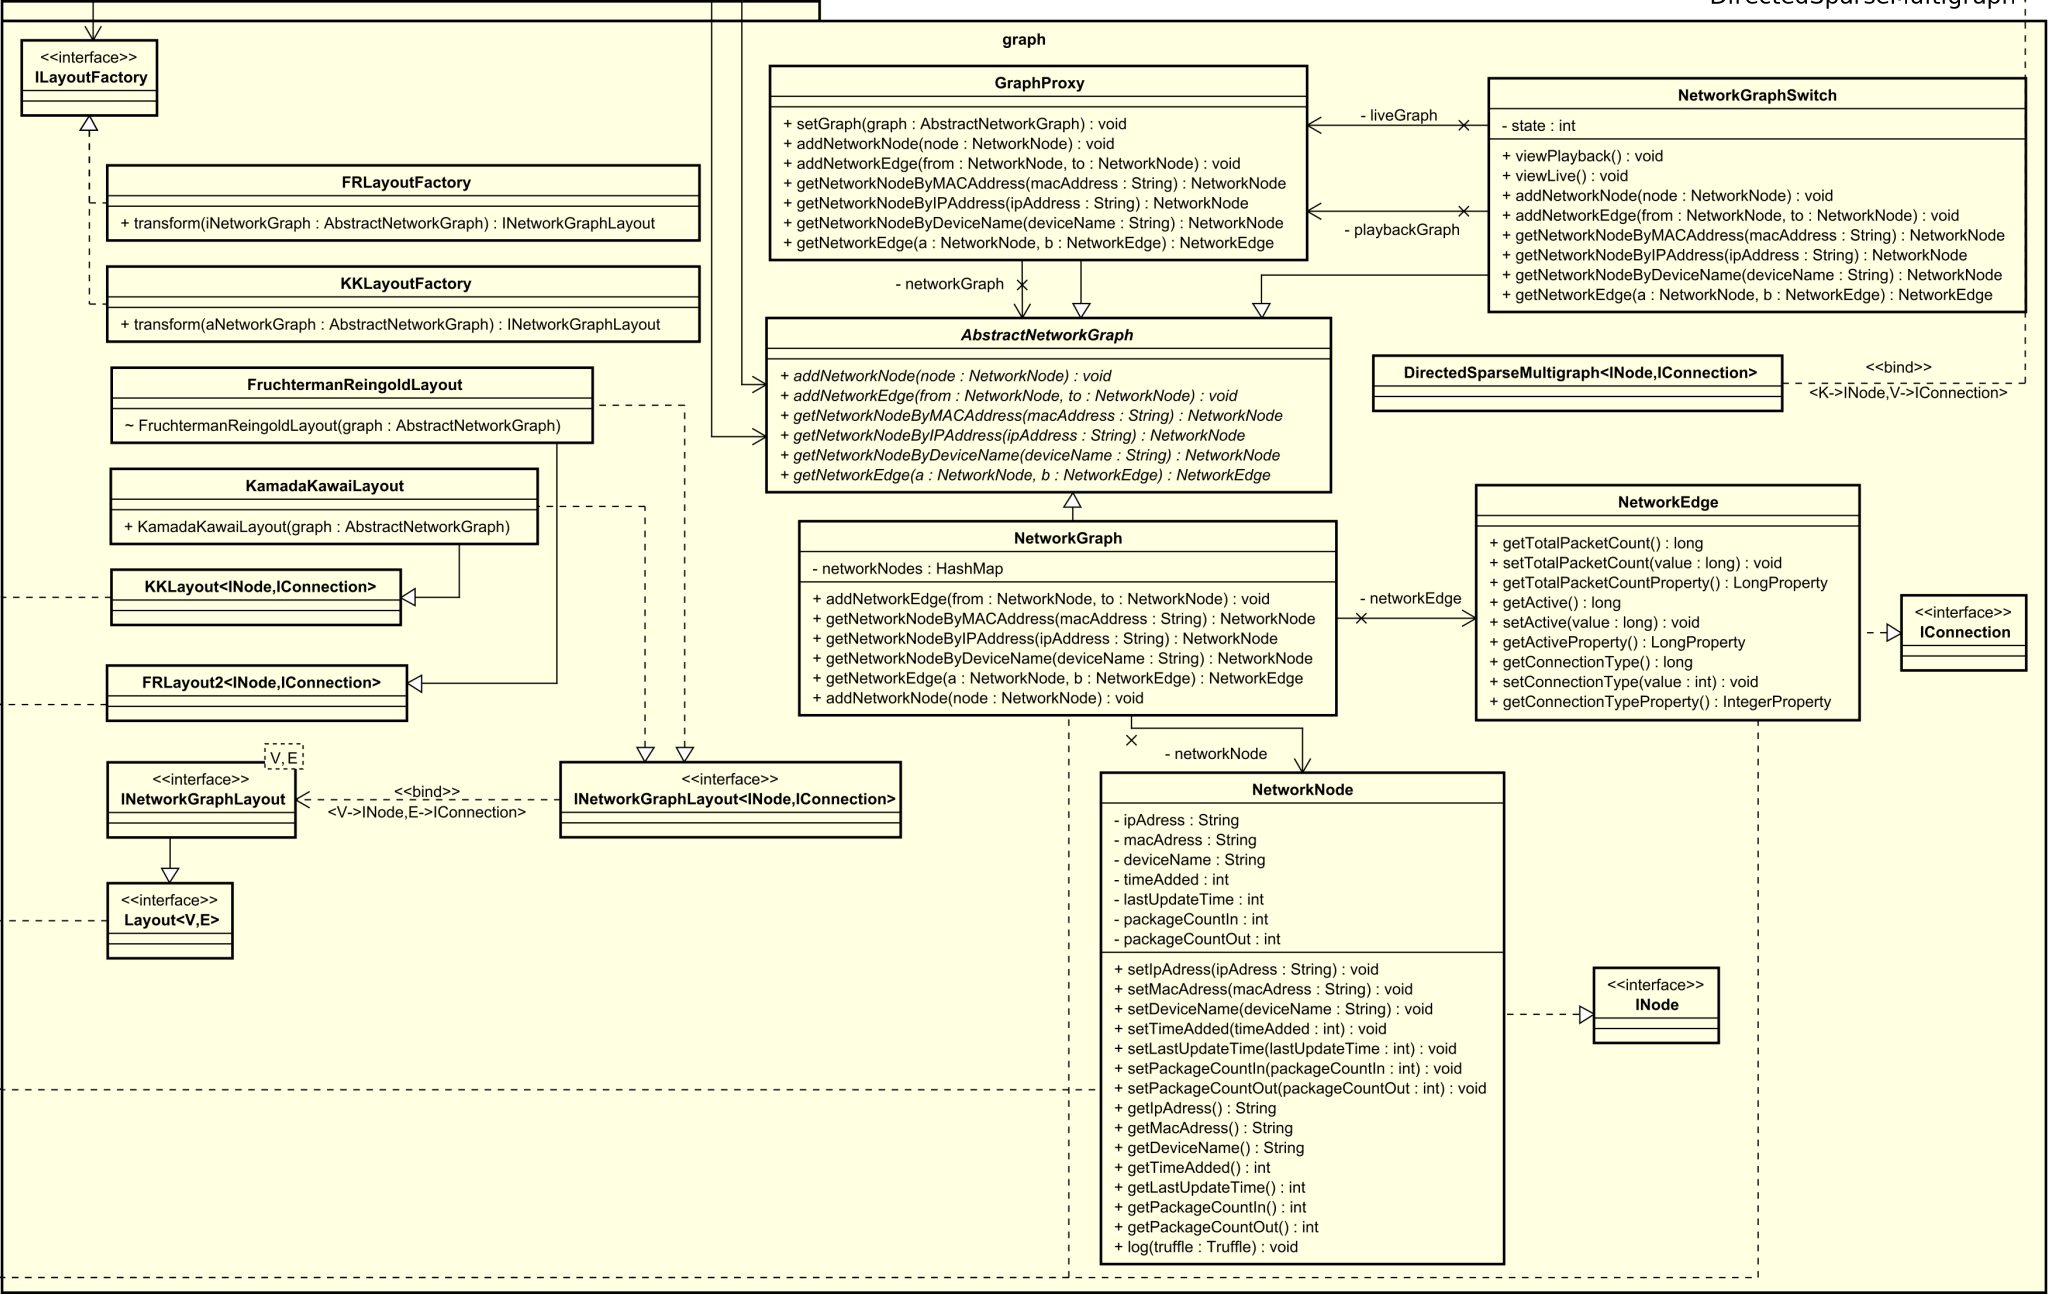
\includegraphics[width=\textwidth]{../diagramimages/graph.png}
      \caption{graph-Package}
    \end{sidewaysfigure}
    \clearpage

    \subsubsection{filter}
    \label{subsubsec:filter}

    \begin{figure}[H]
      \centering
      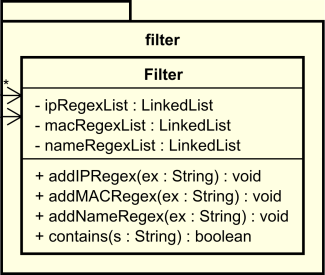
\includegraphics[width=0.8\textwidth]{../diagramimages/filter.png}
      \caption{filter-Package}
    \end{figure}

    \medskip
    Das filter-Package beinhaltet eine \textit{Filter}-Klasse, die in der Lage ist,
    Knoten basierend auf vom Nutzer gesetzen Kriterien zu klassifizieren. Verschiedene
    Klassifikationen werden verschieden in der \gls{gui} dargestellt. So kann
    Beispielsweise eine Blacklist oder Whitelist erstellt werden.
    Natürlich kann der Benutzer basierend auf \gls{ip}- und \gls{mac}-Addressräumen,
    Gerätenamen oder Knotenselektionen seine eigenen Filter definieren.

    \subsubsection{configdata}
    \label{subsubsec:configdata}

    \begin{figure}[H]
      \centering
      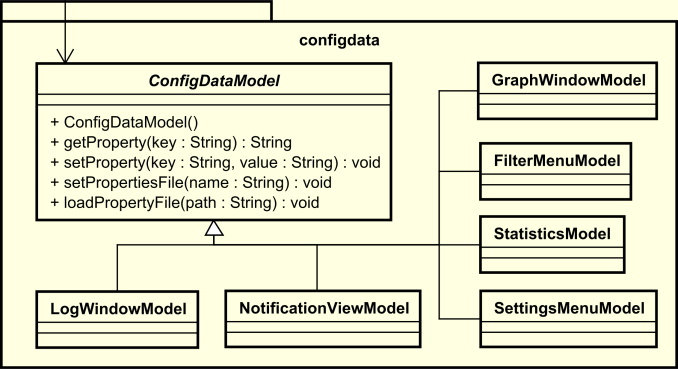
\includegraphics[width=\textwidth]{../diagramimages/configdata.png}
      \caption{configdata-Package}
    \end{figure}

    \medskip
    Im configdata-Package werden jegliche Konfigurationen gespeichert, hin von den
    Beschriftungen der Bedienelemente in der \gls{gui} bis zu den erstellten Filterlisten. Dieses
    wird zum Großteil durch Java Property Files gemacht, welche den Vorteil haben, dass
    sie mit Java Propertyobjekten gekoppelt sind und dadurch leicht auszutauschen sind.
    Das heißt, wenn der Benutzter beispielsweise die Sprache des Programms ändern
    will, so muss intern nur eine andere Property File geladen werden.
    \newline
    \newline
    Der Aufbau dieses Packages setzt sich aus einer abstrakten Oberklasse
    \textit{ConfigDataModel} zusammen, die das Zusammenspiel zwischen Property Files
    und Propertyobjekten verwaltet. Jedes \gls{gui}-Element, welches Daten anzeigt, hat
    ein JavaFX Property-Binding mit einer Unterklasse, die \textit{ConfigDataModel}
    bererbt. So wird automatisch die \hyperref[subsec:view]{View} aktualisiert,
    wenn sich das darunterliegende ConfigDataModel-Objekt ändert. D.h.
    \textit{FilterMenuModel} beinhaltet alle Konfigurationsdaten inklusiver der
    Filterlisten des Filtermenüs. Das Gleiche gilt für alle anderen Menüs und
    deren Models.


    \subsubsection{truffledatalog}
    \label{subsubsec:graphlog}

    \begin{figure}[H]
      \centering
      \includegraphics[width=0.5\textwidth]{../diagramimages/truffledatalog.png}
      \caption{turffledatalog-Package}
    \end{figure}

    \medskip
    Das truffledatalog-Package beinhaltet eine \textit{TruffleLogger}-Klasse, von
    welcher jeder Knoten eine Instanz besitzt. Diese wird beim Eintreffenden neuer Truffles
    (oder Commands) benutzt um die neuen Daten des \glspl{truffle} in einer Text- oder xml-Datei zu speichern,
    sodass bei Bedarf genau gesehen werden kann, was für \glspl{paket} bei einem
    Knoten eingetroffen sind. D.h., dass jeder Knoten seine eigene Text- oder xml-Datei
    hat, wo genau drin steht was für \glspl{paket} dieser schon erhalten hat,
    von wem, etc.


\subsection{view}
\label{subsec:view}

Das view Package enthält alle Klassen, die für die Graphishe Benutzeroberfläche vonnöten sind.

\clearpage
\begin{sidewaysfigure}
  \centering
  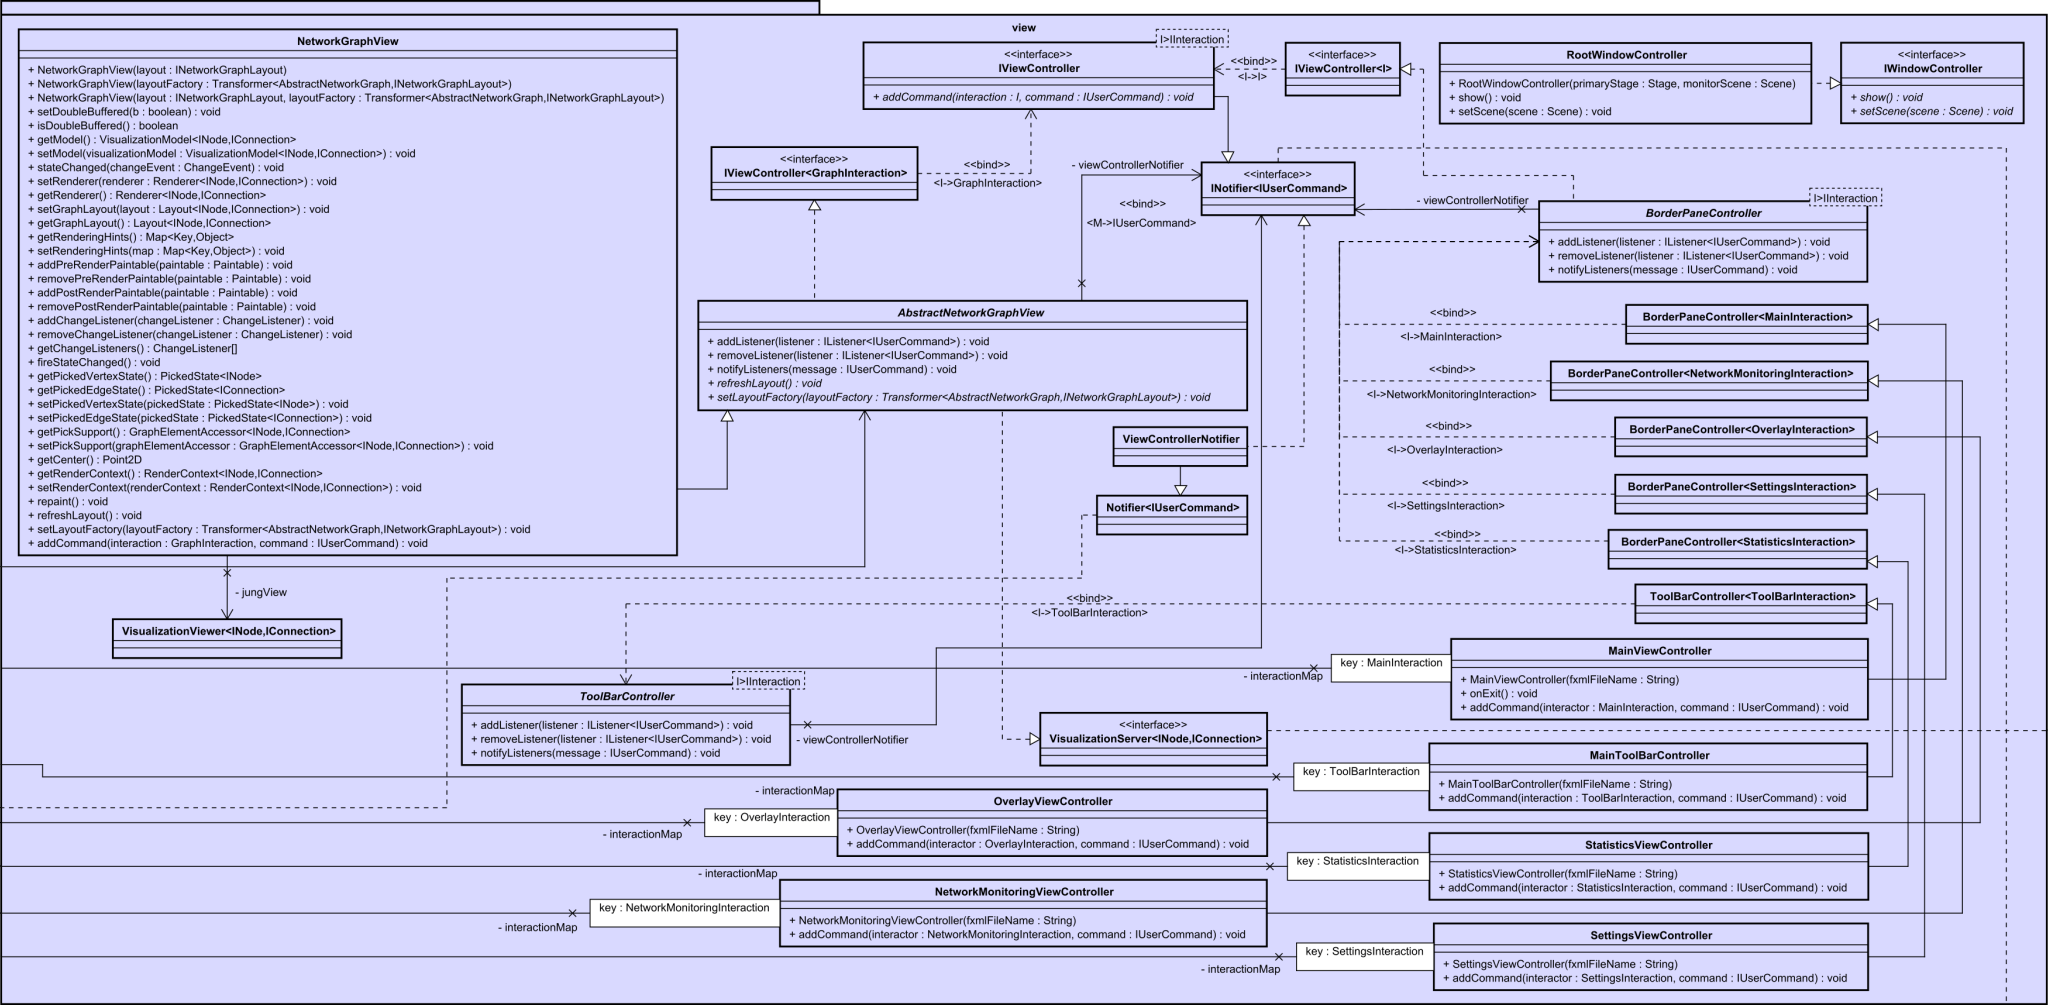
\includegraphics[width=\textwidth]{../diagramimages/view.png}
  \caption{replaylogging-Package}
\end{sidewaysfigure}
\clearpage


\begin{frame}{interaction}
  \begin{figure}
    \centering
    \includegraphics[width=0.8\textwidth]{./images/interaction.png}
  \end{figure}
\end{frame}


\medskip

